\documentclass{article}

\usepackage[margin=1in]{geometry} % Set margins to 1 inch
\usepackage{graphicx} % Allows including images
\usepackage{float} % Allows for precise placement of figures
\usepackage{amsmath} % Allows for math equations
\usepackage{siunitx} % Allows for SI units
\usepackage{placeins} % Makes sure images are in their respective sections by \FloatBarrier

\begin{document}

\title{Hardware Assignment Report}
\author{Saketh Ram Kumar Dondapati(AI22BTECH11023)}
\date{}
\maketitle

\section{Aim}
To make a Random Number Generator using Shift Generators

\section{Components}
\begin{enumerate}    
    \item Breadboard
    \item Seven Segment Display : Common Anode
    \item Seven Segment Display Decoder [7447]
    \item FlipFlop [7474] x2
    \item XOR gate [7486]
    \item 555 IC
    \item Resistors [10M$\Omega$, 1K$\omega$ x2]
    \item Capacitors [47nF,470nF]
    \item USB micro B breakout board
    \item Jumper wires
\end{enumerate}

\begin{figure}[ht]
        \centering
        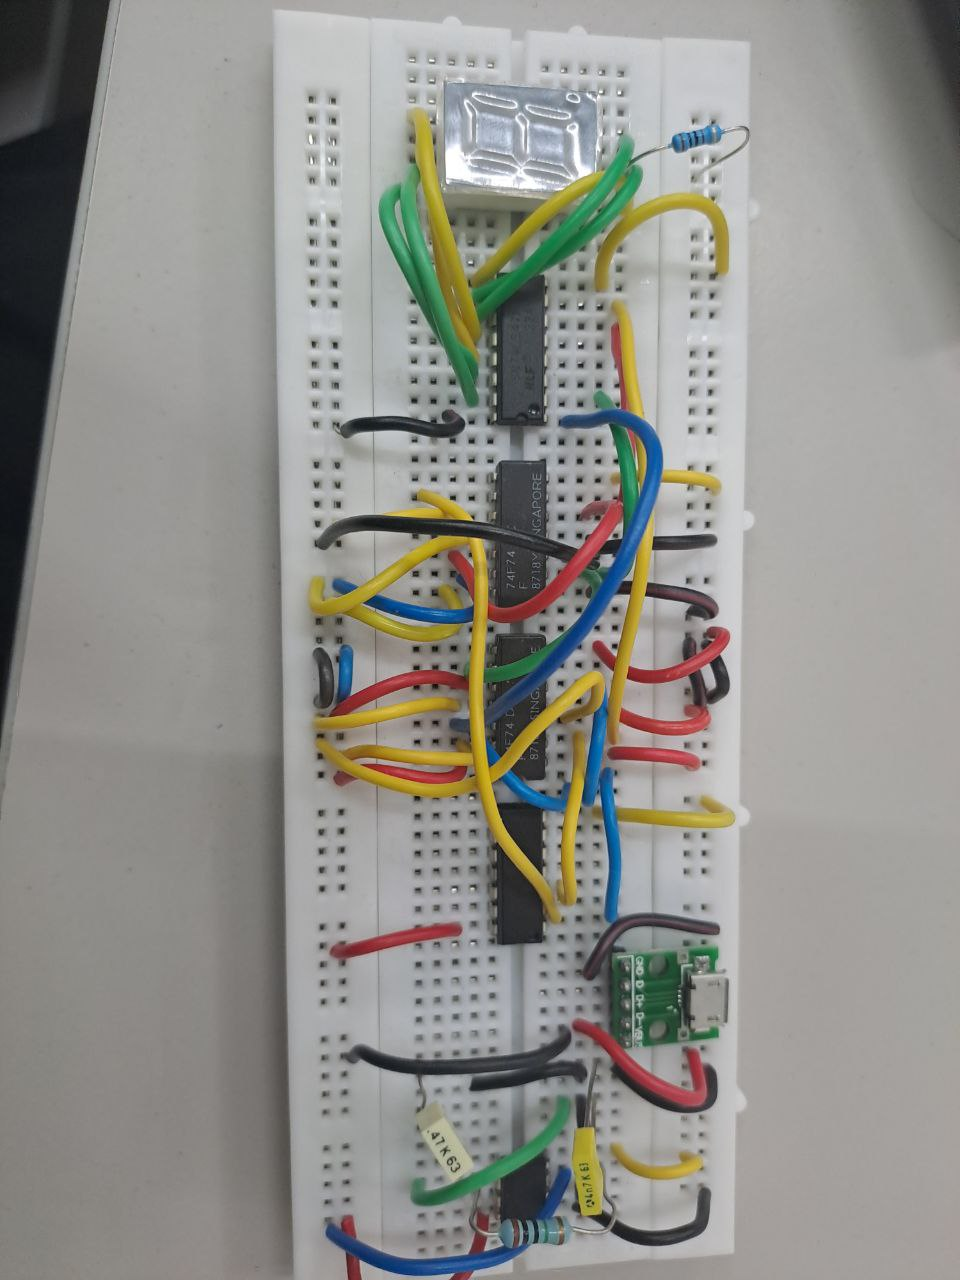
\includegraphics[width=1\linewidth]{projimage.jpg}
        \caption{Circuit Board}
        \label{fig:view}
\end{figure}

\section{Description}
The given circuit is a visual representation of how randon variables can be connected to signal processing.
When considering the usage of a circuit with a seven-segment display in relation to random variables, it typically involves generating random numbers and displaying them on the seven-segment display. Random variables are variables whose values are determined by chance or probability.

\subsection{Overview}
The Flip Flofs take the input and based on that outputs are generated. The generated outputs are random and the numbers shown are from 1 to 15. The randomness is predictable because this system is deterministic.a deterministic system is a system in which no randomness is involved in the development of future states of the system.\\
The order of the output in this case follows : 1, 3, 7, 15, 14, 13, 10, 5, 11, 6, 12, 9, 2, 4, 8

\section{Block Diagram}
\begin{figure}[ht]
        \centering
        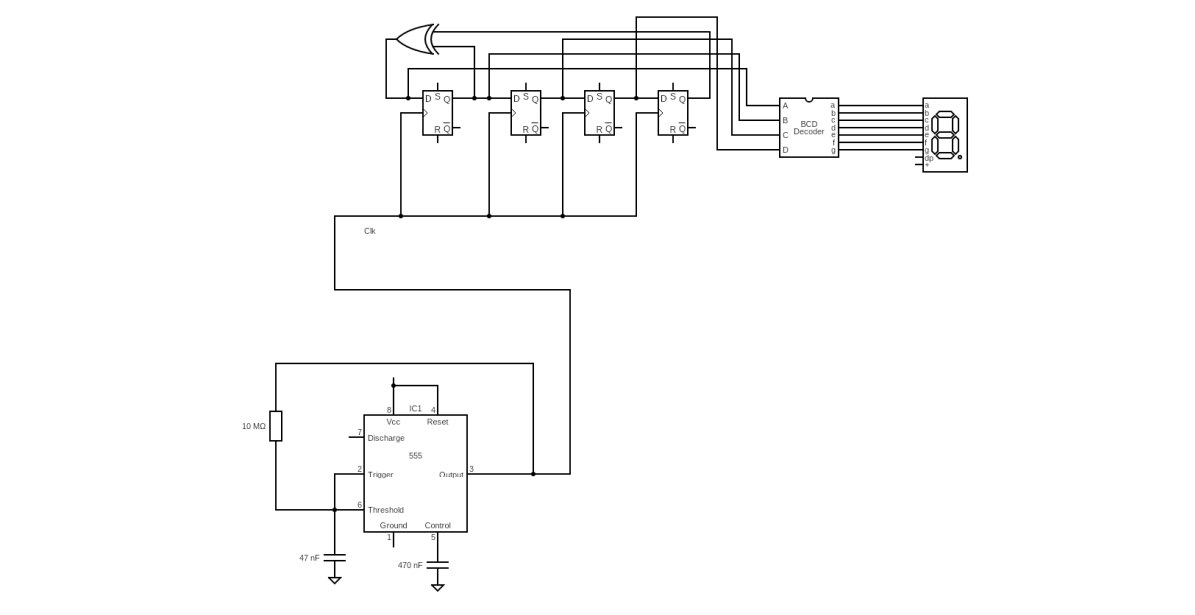
\includegraphics[width=0.8\linewidth]{blockdiag.jpg}
        \caption{Block Diagram}
        \label{fig:view}
\end{figure}

\end{document}
